% !TEX program = xelatex
\documentclass[11pt]{beamer}

\usepackage{unicode-math}
\usepackage{amsmath}
\usepackage{amsfonts}
\usepackage{amssymb}
\usepackage[style=ddmmyyyy]{datetime2}
\usepackage{graphicx}
\usepackage{hyperref}
\usepackage{fontspec}

\makeatletter
\def\input@path{{../../theme/}}
\makeatother

\usetheme{mis}

\setsansfont{Source Sans Pro}[Numbers=OldStyle]
\setmathfont{STIX Two Math}[Scale=MatchLowercase]
\setmonofont{Consolas}[Scale=MatchLowercase]

\author{Lê Thành Văn \texorpdfstring{\\ \footnotesize lt.van@hutech.edu.vn}{}}
\title{Cơ sở dữ liệu ứng dụng}
\date{}
\institute{Khoa Hệ thống thông tin quản lý}
% package setting
\hypersetup {
	colorlinks = true
}
%\usecolortheme{seahorse}
% graphic path
\graphicspath{{../../media/}}

%
\AtBeginSection{
  \frame{
    \sectionpage
  }
}

\begin{document}
    \begin{frame}
        \titlepage
    \end{frame}

    \section{Giới thiệu môn học}
    \begin{frame}{Mục tiêu}
        \begin{itemize}
            \item Hiểu và vận dụng các kiến thức về ngôn ngữ SQL.
            \item Biết cách sử dụng Microsoft SQL Server.
            \item Có kiến thức cơ bản về Hệ quản trị CSDL phi cấu trúc.
        \end{itemize}
    \end{frame}

    \begin{frame}{Nội dung}
        \begin{itemize}
            \item Tổng quan về cơ sở dữ liệu.
            \item Mô hình thực thể quan hệ.
            \item Mô hình thực thể quan hệ mở rộng.
            \item Mô hình quan hệ.
            \item Đại số quan hệ.
        \end{itemize}
    \end{frame}

    \begin{frame}{Điểm số}
        \begin{itemize}
            \item Điểm quá trình (50\%)
            \begin{itemize}
                \item Điểm chuyên cần (40\%).
                \item Điểm bài tập (60\%).
            \end{itemize}
            \item Điểm cuối kỳ (50\%)
        \end{itemize}
    \end{frame}

    \begin{frame}{Thời khóa biểu}
        \begin{itemize}
            \item Lý thuyết (15 buổi, 3 tiết một buổi)
            \begin{itemize}
                \item Thứ 3 (tiết 1): 18/05/2021 -- 06/07/2021.
                \item Thứ 6 (tiết 1): 21/05/2021 -- 02/07/2021.
            \end{itemize}
        \end{itemize}
    \end{frame}

    \section{Môi trường làm việc}
    \begin{frame}{Phần mềm}
        Microsoft SQL Server 2019.\\
        Microsoft SQL Server Management Studio (SSMS).

        \textit{Lưu ý}: 
        \begin{itemize}
            \item Nếu cấu hình máy không đủ, có thể sử dụng các phiên bản 
            cũ hơn của Microsoft SQL Server.
            \item Nếu có thể sử dụng giao diện command line thì không cần cài đặt SMSS.
        \end{itemize}
        
    \end{frame}

    \begin{frame}{SMSS}
        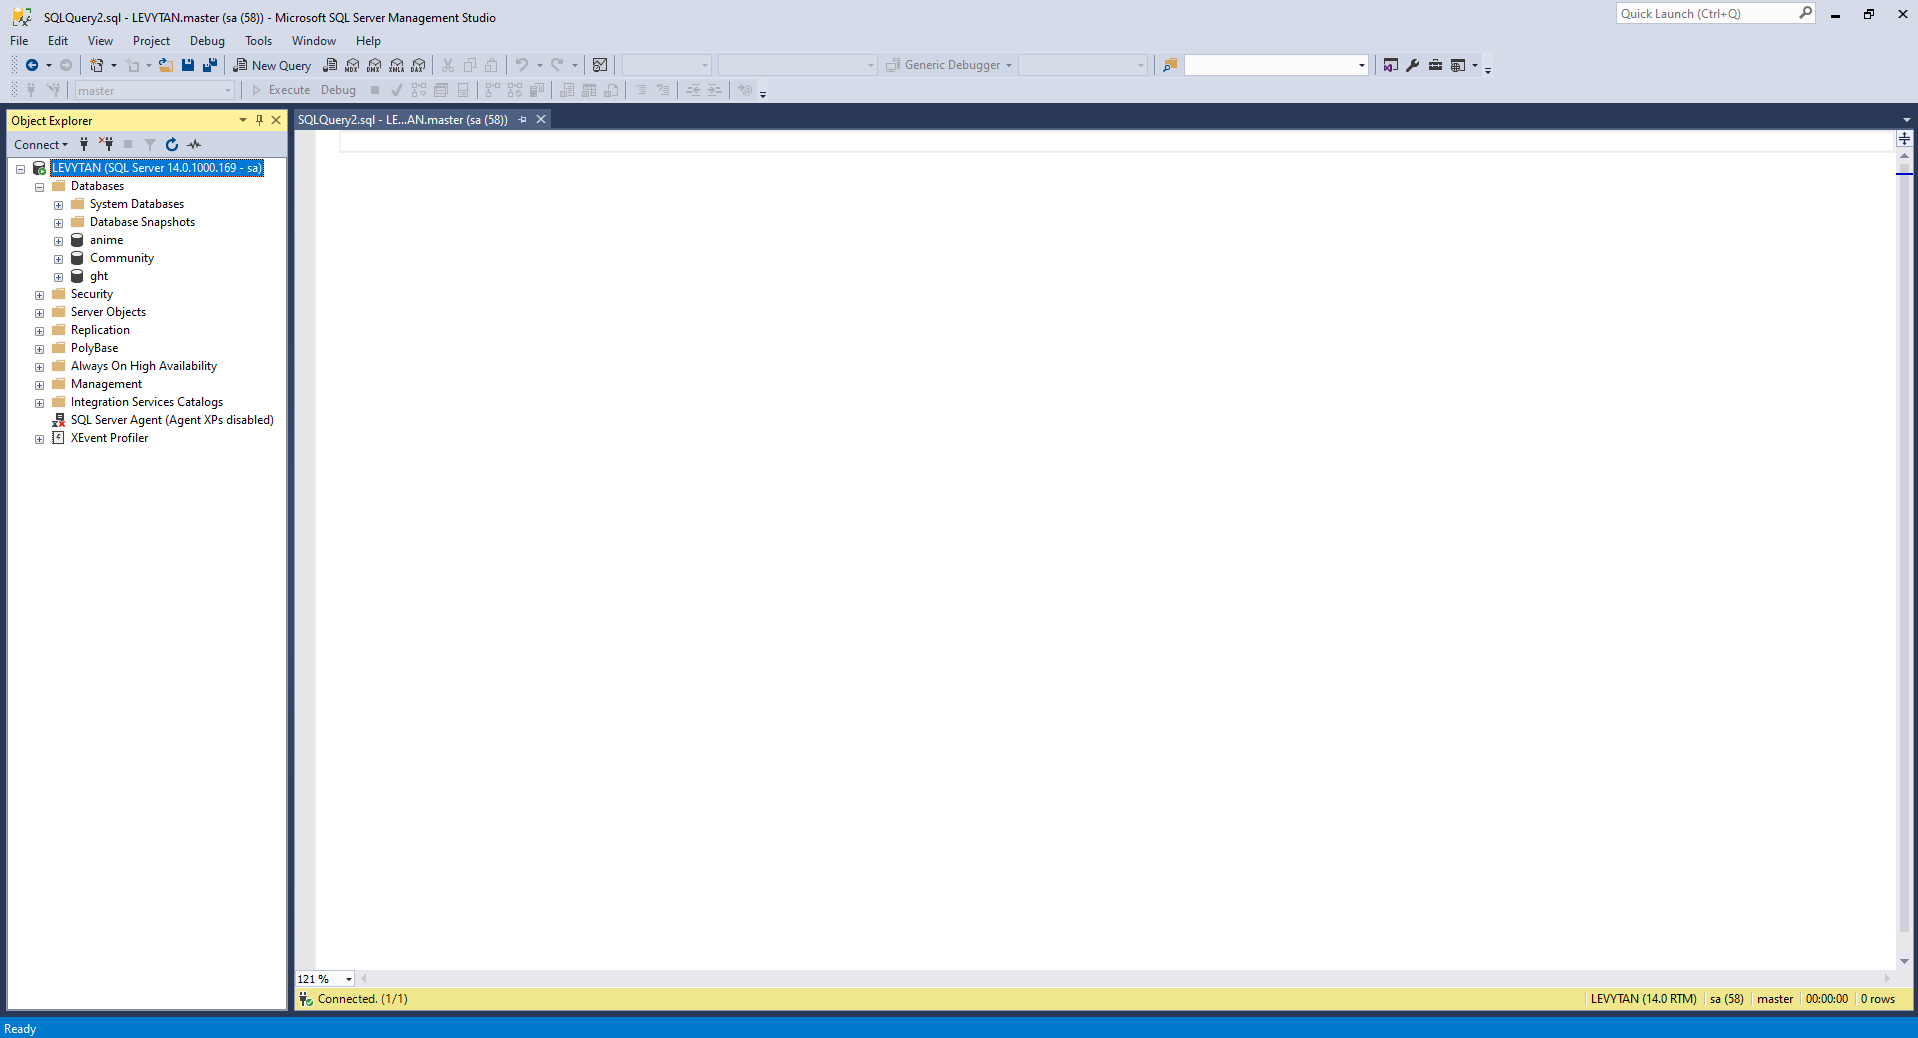
\includegraphics[width=\textwidth]{smss.png}
    \end{frame}

    \section{Tài liệu tham khảo}
    \begin{frame}{Tham khảo}
        \begin{itemize}
            \item \href{https://www.w3schools.com/sql/}{SQL Tutorial}.
            \item \href{https://vietjack.com/sql/}{Hướng dẫn SQL}.
        \end{itemize}
    \end{frame}
\end{document}